\documentclass[man]{apa6}
\title{ECE-5554 Computer Vision: Problem Set 0}
\author{Murat Ambarkutuk \\ murata@vt.edu}
\vfill
\affiliation{Mechanical Engineering Department,\\ Virginia Polytechnic Institute and State University}
\vfill
\note{\today}
\usepackage{listings}
\usepackage{graphicx}
\usepackage{color} %red, green, blue, yellow, cyan, magenta, black, white
\usepackage[inline]{enumitem}   
\makeatletter
% This command ignores the optional argument for itemize and enumerate lists
\newcommand{\inlineitem}[1][]{%
\ifnum\enit@type=\tw@
    {\descriptionlabel{#1}}
  \hspace{\labelsep}%
\else
  \ifnum\enit@type=\z@
       \refstepcounter{\@listctr}\fi
    \quad\@itemlabel\hspace{\labelsep}%
\fi}
\makeatother

\definecolor{mygreen}{RGB}{28,172,0} % color values Red, Green, Blue
\definecolor{mylilas}{RGB}{170,55,241}

\shorttitle{Problem Set 0}
\leftheader{Even-Numbered Page Header}
\begin{document}
\maketitle

\lstset{language=Matlab,%
    %basicstyle=\color{red},
    breaklines=false,%
    morekeywords={matlab2tikz},
    keywordstyle=\color{blue},%
    morekeywords=[2]{1}, keywordstyle=[2]{\color{black}},
    identifierstyle=\color{black},%
    stringstyle=\color{mylilas},
    commentstyle=\color{mygreen},%
    showstringspaces=false,%without this there will be a symbol in the places where there is a space
    numbers=left,%
    numberstyle={\tiny \color{black}},% size of the numbers
    numbersep=12pt, % this defines how far the numbers are from the text
    emph=[1]{for,end,break},emphstyle=[1]\color{red}, %some words to emphasise
    %emph=[2]{word1,word2}, emphstyle=[2]{style},    
}

\section*{Matlab Code}

\section{Answer Sheet}
\subsection{Short answer problems}
	\begin{enumerate}
		\item Completed.
		
		\item 
			\begin{enumerate}
				\item Creates a row vector containing random permutations of numbers between 1 and 1000.
				
				\item Line 1: Creates a matrix: \\
					\[ a= \left[ \begin{array}{ccc}
					1 & 2 & 3 \\
					4 & 5 & 6 \\
					7 & 8 & 9 \end{array} \right]\] 
					Line 2 assigns the second row of x to the variable b.
					$$b = [4,5,6]$$

				\item Creates a matrix: \\
					\[ a= \left[ \begin{array}{ccc}
					1 & 2 & 3 \\
					4 & 5 & 6 \\
					7 & 8 & 9 \end{array} \right]\] 
					Line 2 assigns the all the values the variable b in column vector form.
					$$b= [\begin{array}{c c c c c c c c c}1, & 4, & 7, & 2, & 5, & 8, & 3, & 6, & 9 \end{array}] '$$

				\item Line 1 creates the column vector $f$ [1$\times5$] with the normally distributed random values. \\
					Line 2 sets another variable and fills it with the elements of f which are above 0.

				\item Line 1 sets a row vector  [1$\times10$] with zeros and adds 0.5 to each element of it.
					$$x = [0, 0, 0, 0, 0 ,0 , 0, 0, 0, 0] + 0.5$$
					$$x= [0.5, 0.5, 0.5, 0.5, 0.5, 0.5, 0.5, 0.5, 0.5, 0.5]$$
					Line 2 creates another row vector with the same size of vector x [1$\times10$], and multiplies each element of new row vector with 0.5. \\
					$$y = [1, 1, 1, 1, 1 , 1, 1, 1, 1, 1] \times 0.5$$
					$$y= [0.5, 0.5, 0.5, 0.5, 0.5, 0.5, 0.5, 0.5, 0.5, 0.5]$$
					Line 3 sums vector x and y and assigns the result to z.
					$$z = x + y$$
					$$z= [1, 1, 1, 1, 1, 1, 1, 1, 1, 1]$$
					
				\item Line 1 creates a row vector [1$\times100$] which contains the sequence starting from 1 to 100 (inclusive).
					$$a= [1,2,3,4 \dots 98,99,100]$$
					Line 2 flips the vector and sets vector b with these values.
					$$a= [100,99,98,97 \dots 3,2,1]$$	
			\end{enumerate}
		
		\item The code is in PS0\_1-3.m file.
			\begin{enumerate}
				\item The function returning n trials of 6-sided dice roll is given below. (Please find the diceTrials.m file .zip file.)
				The contents of diceTrials.m: \\
				\lstinputlisting{diceTrials.m}
				\item \inlineitem \inlineitem \inlineitem  \lstinputlisting{PS0_1_3.m}
			\end{enumerate}
			
		\item The code is in PS0Q1.m file. \\
			The source matrix created and used as input file is depicted below. \\
			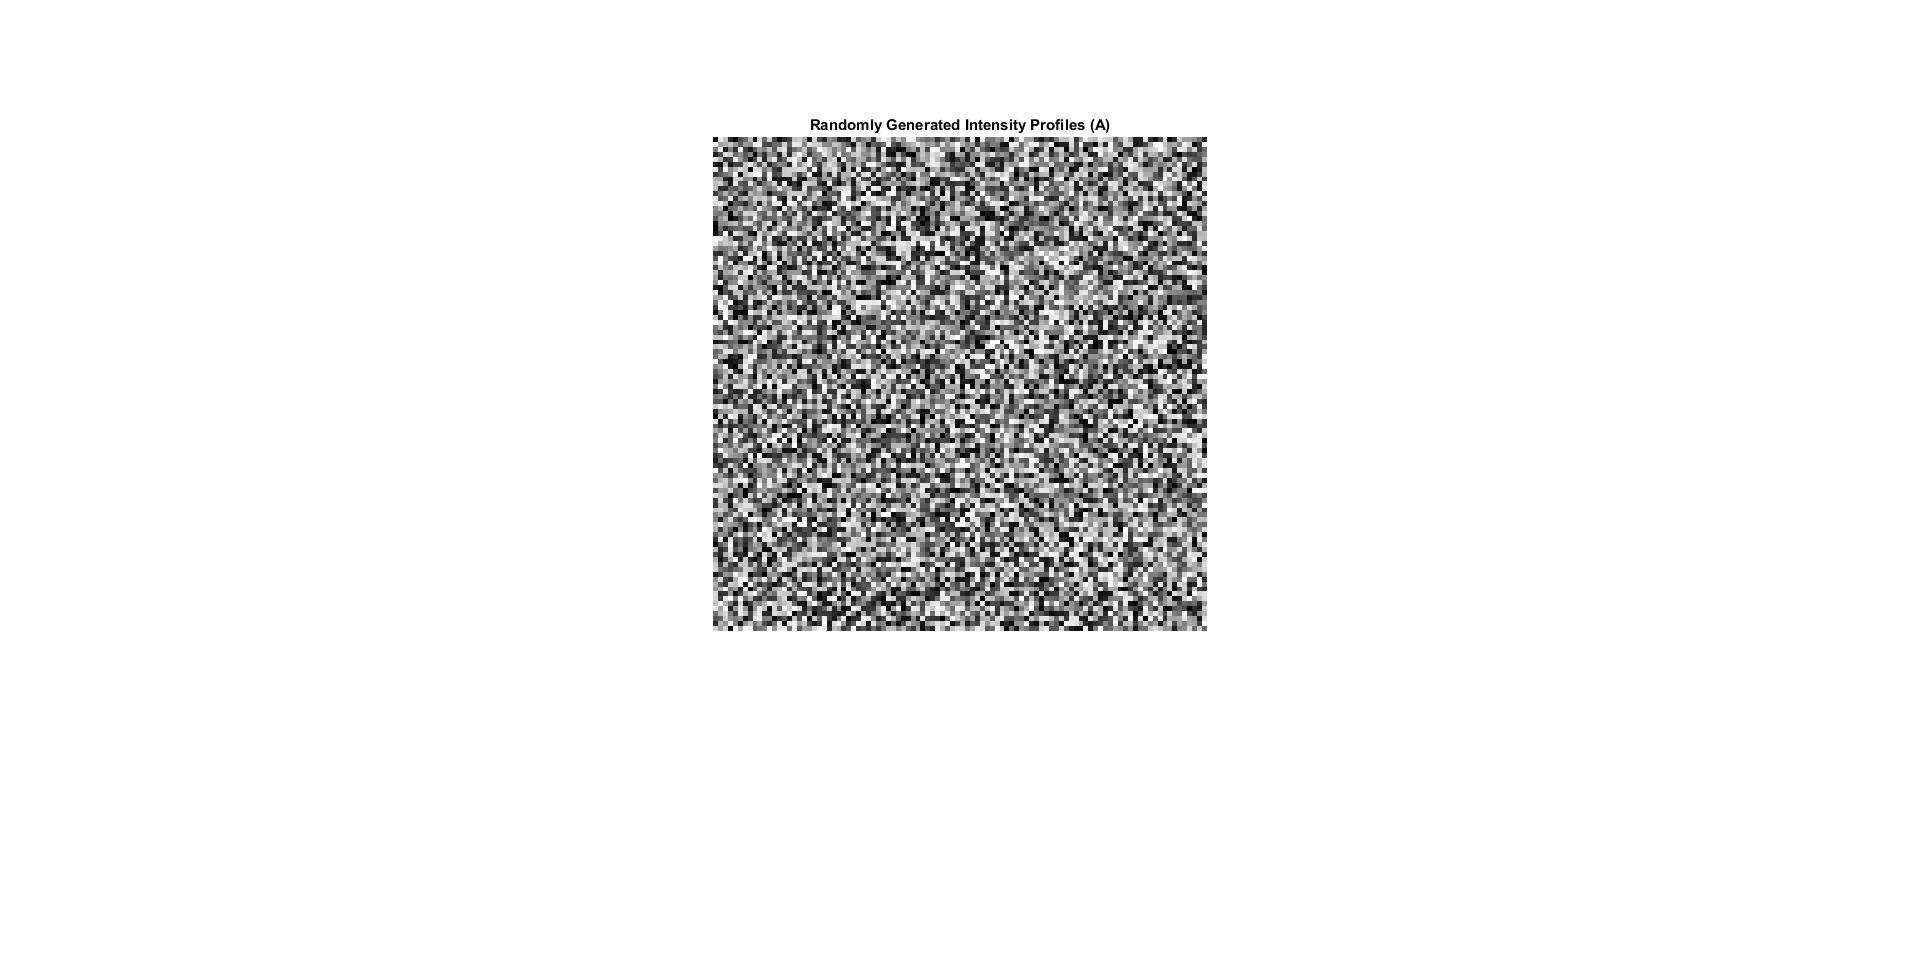
\includegraphics[width=\linewidth]{plots/1-A-4/a.png}
		
			\begin{enumerate}
				\item Result of sort process.
					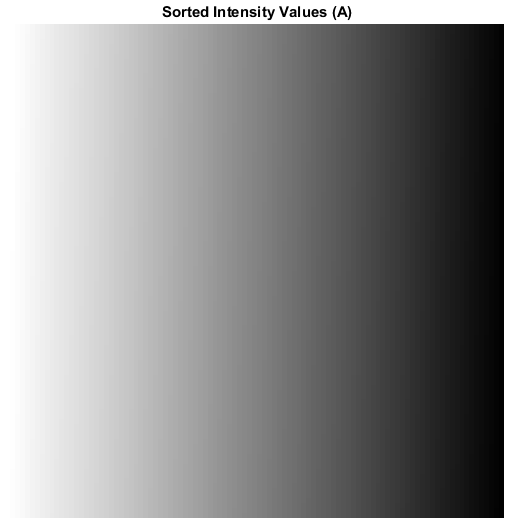
\includegraphics[width=\linewidth]{plots/1-A-4/a_sorted.png}
			
				\item Intensity histogram of A is given below.
					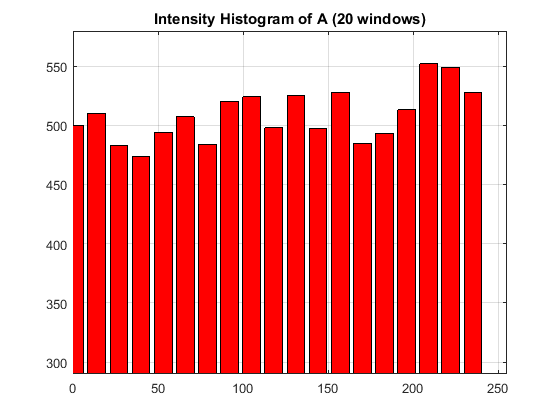
\includegraphics[width=\linewidth]{plots/1-A-4/b.png}
				
				\item The bottom left quadrant of A is depicted below. Please also find the attached outputXPS0Q1.mat in the zipped folder.
					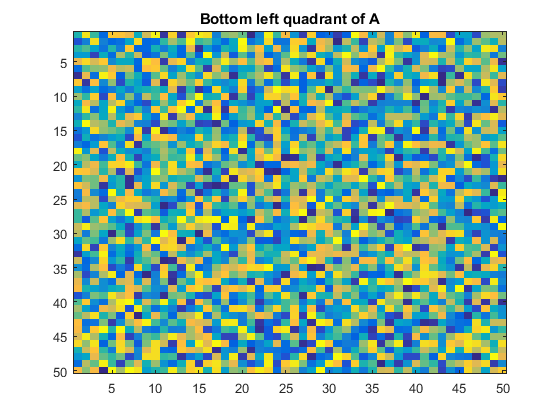
\includegraphics[width=\linewidth]{plots/1-A-4/c.png}
					
				\item Please find the attached outputYPS0Q1.mat file.
					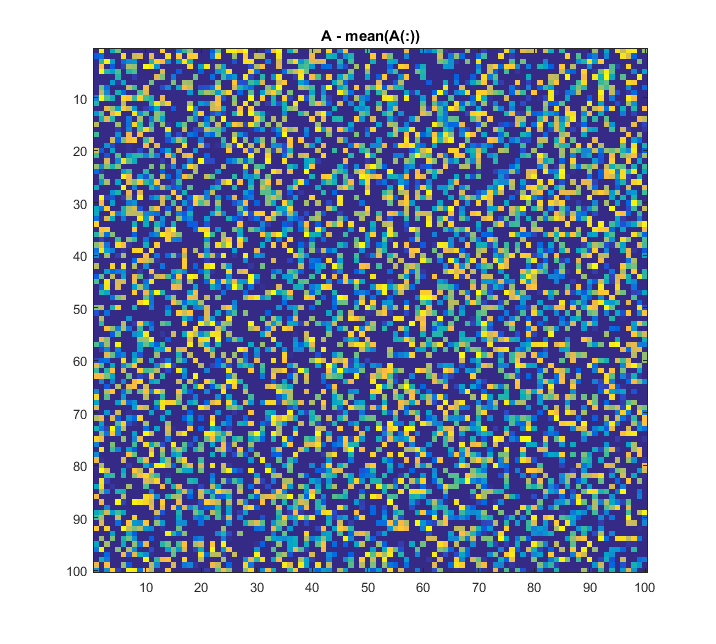
\includegraphics[width=\linewidth]{plots/1-A-4/d.png}
					
				\item Since the first matrix $A$ is randomly created in $uint8$ data class $[0-255]$, pixels appear the same when the frame is displayed with imagesc() and imshow(). Hence, they both give the same output. Please find the attached outputYPS0Q1.mat file.
					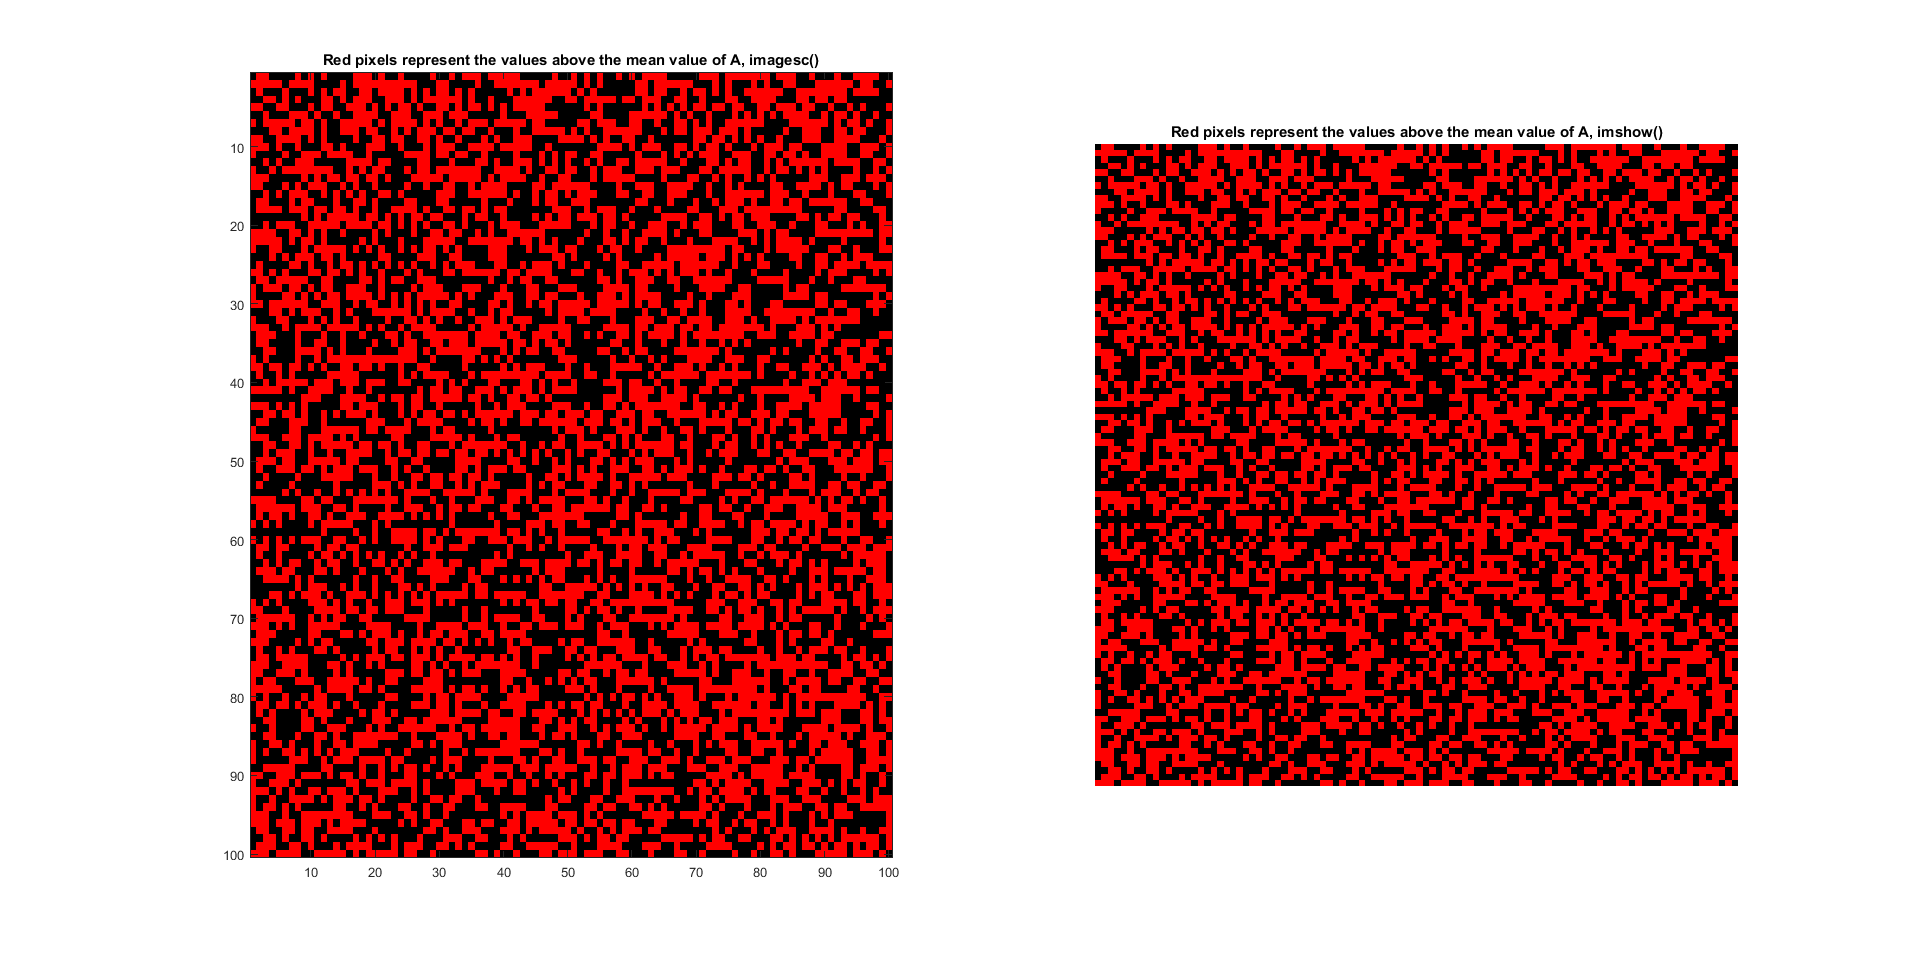
\includegraphics[width=\linewidth]{plots/1-A-4/e.png}
				The contents of PS0Q1.m: \\
				\lstinputlisting{PS0Q1.m}
			\end{enumerate}
		
	\end{enumerate}

\subsection{Short Programming Question}
	Input image: 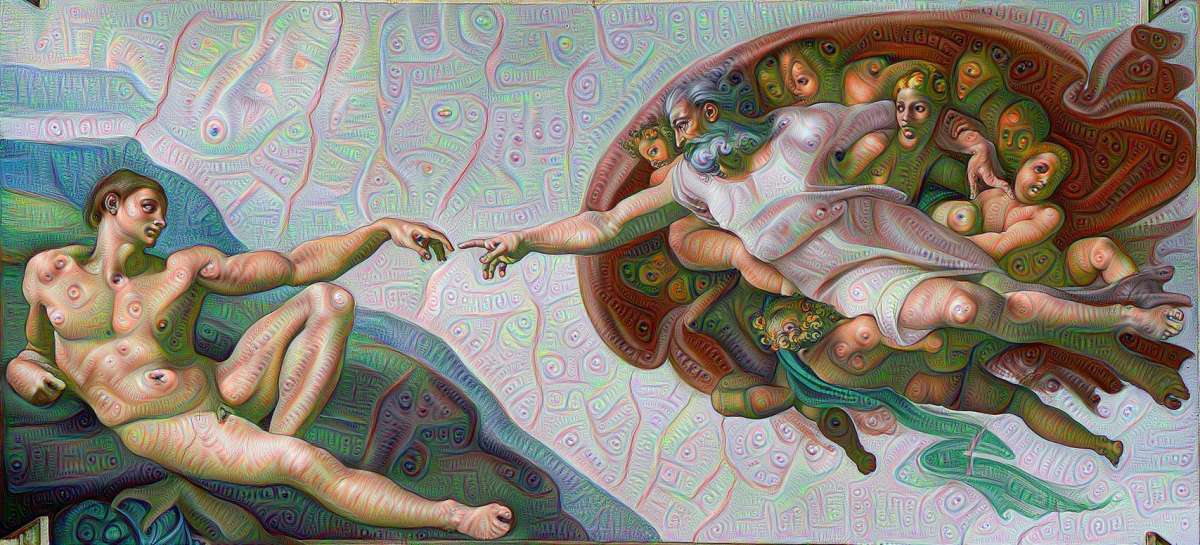
\includegraphics[width=\textwidth]{plots/2/inputPS0Q2.jpg}
	Results: 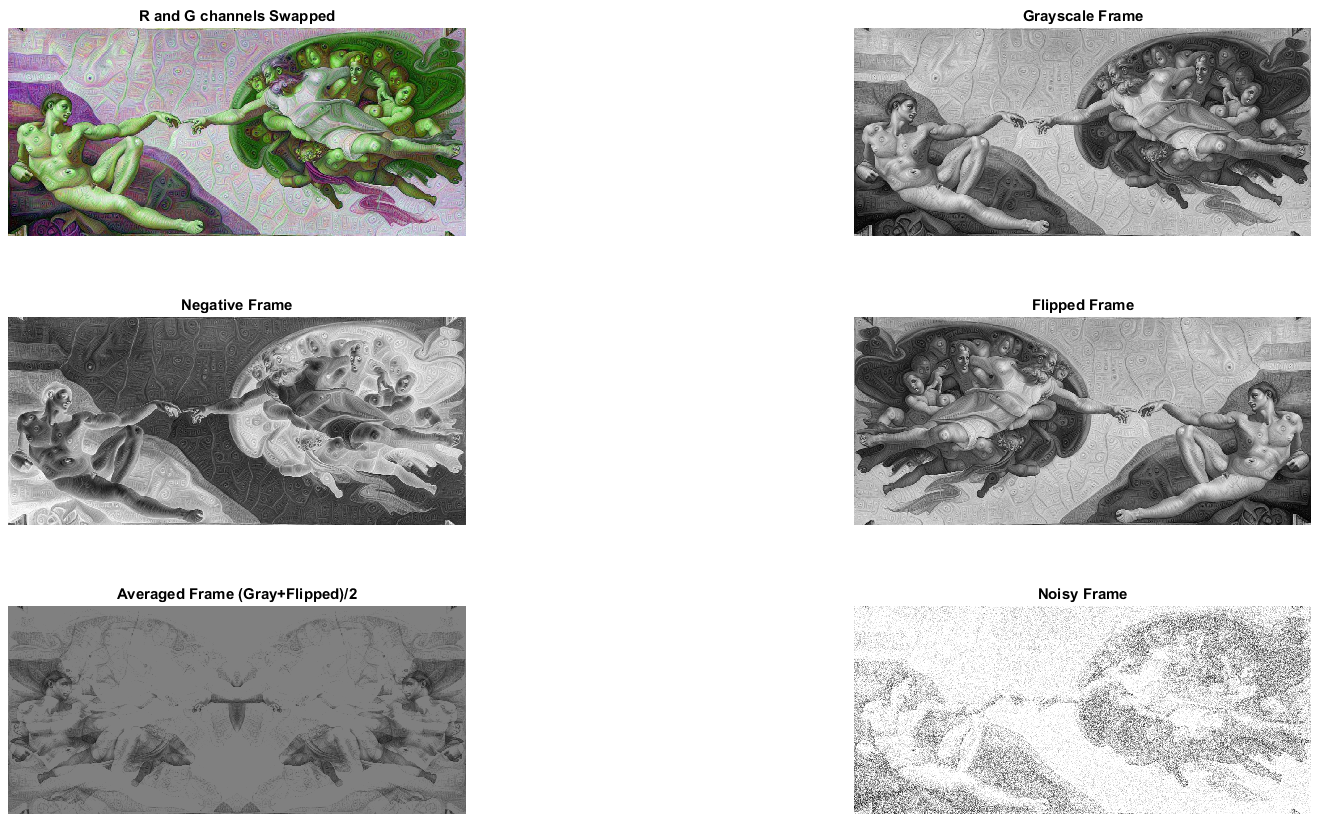
\includegraphics[width=\textwidth]{plots/2/subplot.png}
	\begin{enumerate}
		\item 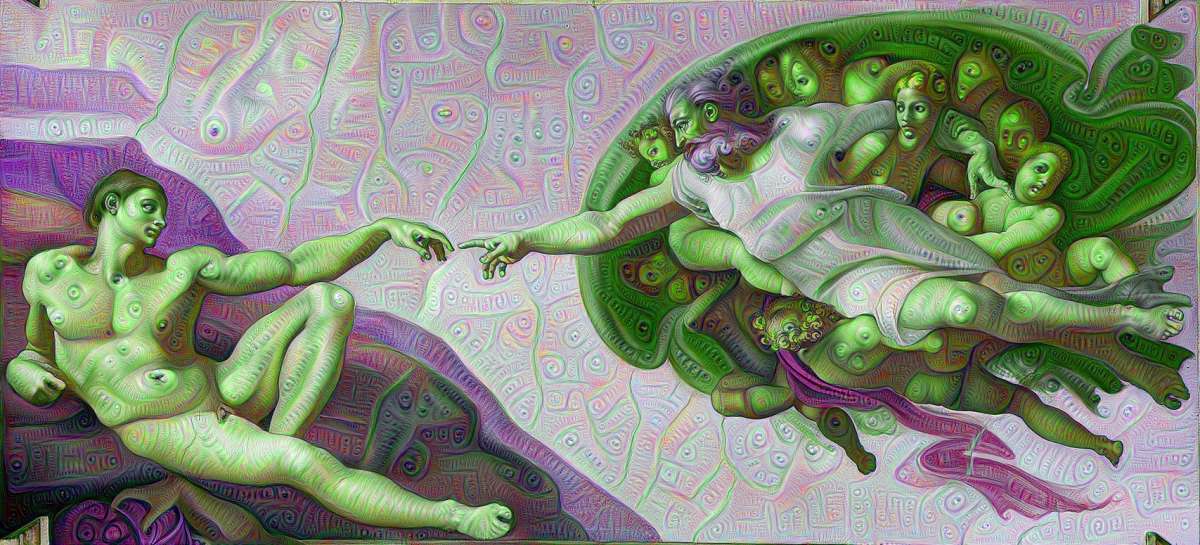
\includegraphics[width=\textwidth]{plots/2/swapImgPS0Q2.png}
		\item 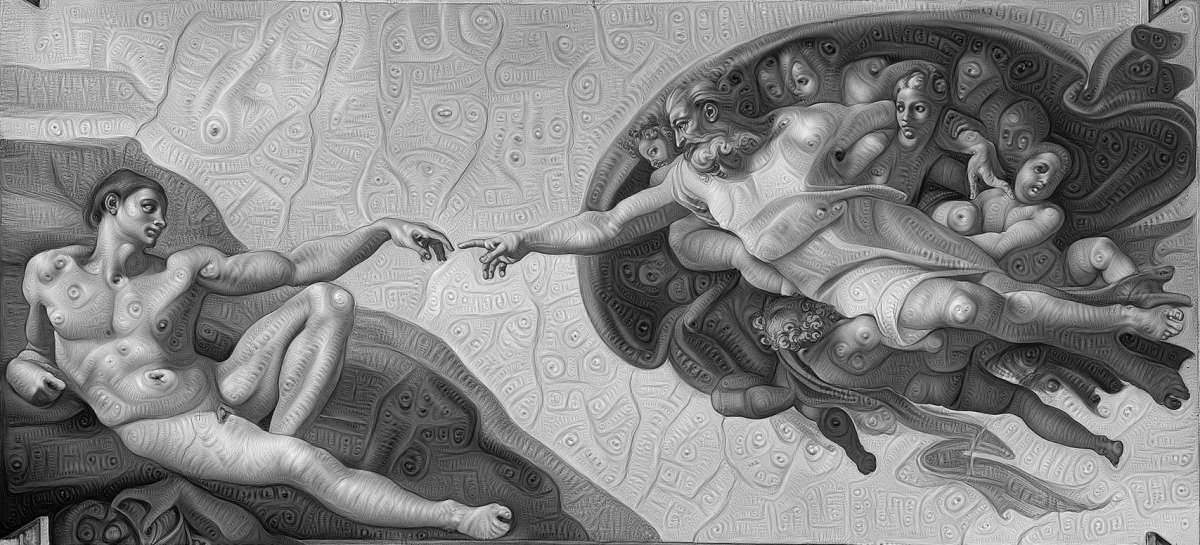
\includegraphics[width=\textwidth]{plots/2/grayImgPS0Q2.png}
		\item
			\begin{enumerate}	
				\item 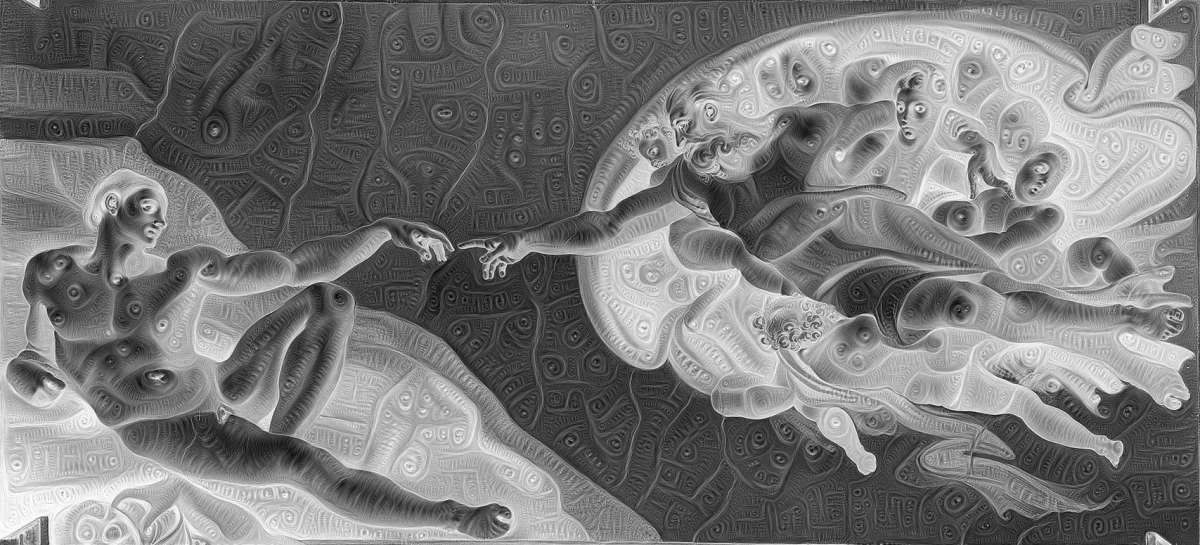
\includegraphics[width=\textwidth]{plots/2/negativeImgPS0Q2.png}
				\item 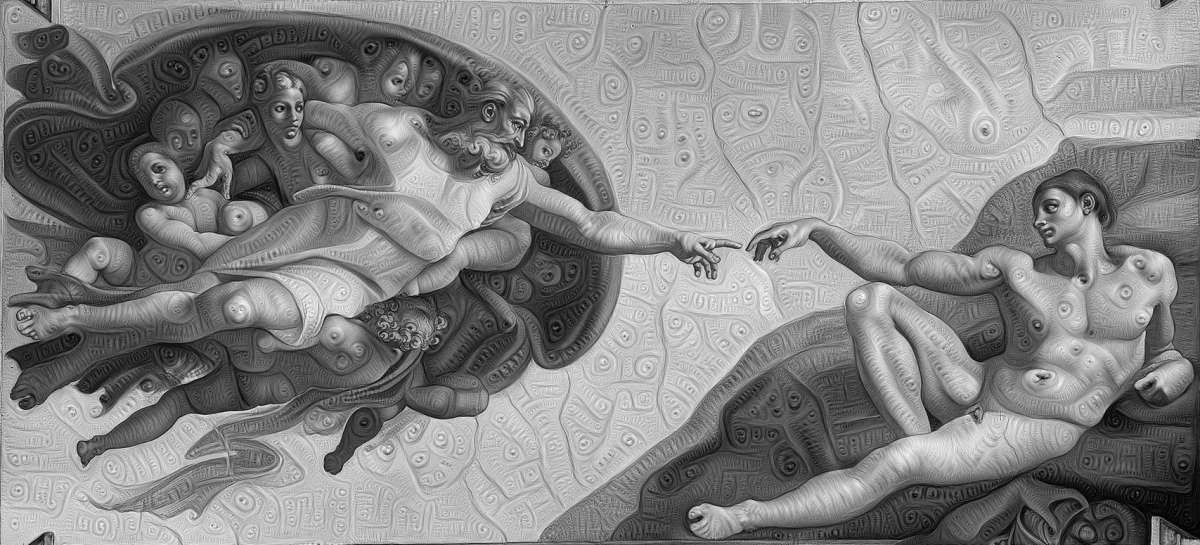
\includegraphics[width=\textwidth]{plots/2/mirrorImgPS0Q2.png}
				\item 
\includegraphics[width=\textwidth]{plots/2/avgImgPS0Q2.png}
				\item Because all the operations was completed with $uint8$ data class, any pixel going above 255 or below 0 automatically thresholded. \\
					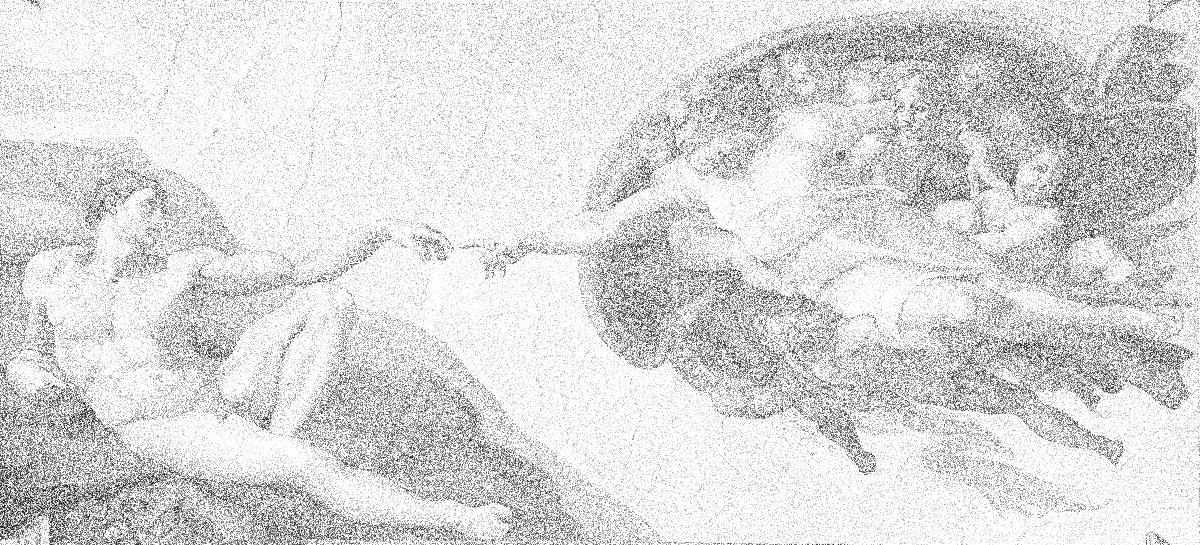
\includegraphics[width=\textwidth]{plots/2/addNoiseImgPS0Q2.png}
			\end{enumerate}
		The contents of PS0Q2.m: \\
		\lstinputlisting{PS0Q2.m}
	\end{enumerate}
\end{document}
